%卒業論文用テンプレート
\documentstyle[graphicx]{jronbun}


%諸定義
\newenvironment{indention}[1]{\par
\addtolength{\leftskip}{#1}
\begingroup}{\endgroup\par}

%論文名
\title{3密回避のための室内環境情報の能動的提供機能の開発}
%教官名
\kyoukan{高橋寛教授}
\second{王森レイ講師}
%名前
\author{小田 恵吏奈}
%提出日
\date{令和3年2月17日提出}
%講座名
\kouza{\gt 愛媛大学工学部情報工学科情報システム工学講座}

\begin{document}
	%タイトル生成
	\maketitle
	%目次生成
	\pagenumbering{roman}
	\tableofcontents
	\cleardoublepage
	\pagenumbering{arabic}
	
	%--ここから本文--
	%第1章 まえがき
	\chapter{まえがき}
	%第1章 まえがき

%1章1節
\section{研究背景および目的・目標}
近年では,IoT(Internet of Things)の普及が進んでおり,様々なものがインターネットに繋がる時代である.インターネトに繋がるものをIoT機器(IoTデバイス)といい,例として家電や自動車・産業用ロボットなどが挙げられる.
IoTを実現する上で,周囲の情報を検知するセンシングデバイスやネットワークは必要不可欠である.
そして,センシングデバイスがインターネットに繋がることで,外部の悪意のある第三者からの攻撃により,データを盗聴・改ざんする恐れが懸念される.

第三者からの攻撃事例に,タイヤ空気圧監視システムへの攻撃事例がある\cite{maegaki}.
タイヤ空気圧監視システム(TPMS:(Tire Pressure Monitoring System))とは,
タイヤの空気圧を常時監視するシステムであり,空気圧が低いタイヤで高速走行をすることによるタイヤバースト事故を防ぐ効果が期待される.
しかし,このTPMSの無線通信には脆弱性があることが問題となっている.
その問題の一つとして,TPMSでは通信メッセージが暗号化されていないため,盗聴解析が容易になるという点がある.
また, TPMSの空気圧報告メッセージになりすますことができるという問題点もある.
この事例から,センシングデバイスにおいて,ネットワーク上の脆弱性があることで外部からの攻撃によるデータの盗聴・改ざんが行われてしまうリスクがあることから,セキュリティ対策が不可欠となることが分かる.

センシングデバイスのセキュリティ対策の一つに認証・暗号化がある.
しかしながら,AESなど従来の暗号化方式は処理負荷が高いことから処理性能の低いセンシングデバイスには導入困難であるため,現在市場に出回っているセンシングデバイスには認証・暗号化といったセキュリティ対策が不十分で,脆弱性があると考えられる.
そこで,センシングデバイスなど,処理性能の低いIoT機器において,
極めて小さい処理負荷で認証と暗号化通信のできる軽量なセキュリティ対策が求められる.

本研究では,処理能力の低いセンシングデバイスで構成されるIoTシステムにおいて,デバイスとエッジサーバー間の
安全なデータ通信を行うセキュアな組込みシステムを開発することを目的とする.
具体的には,高知工学科大学の清水明宏教授が処理能力の低い装置へのセキュリティ機能実装のために
開発されたワンタイムパスワード認証方式SAS-L2をIoTセンシングデバイス
に実装することで,デバイス間の相互認証およびセンシングデータの暗号化通信方法を実現する.
なお,本研究は,2人チーム(浅野美咲,内山田隆太)でV字開発モデルに従って処理能力の低いセンシングデバイスで構成されるSAS-L2認証を導入したセキュアなIoTシステムの開発を行う.
システムの設計にはUMLを利用する.
チームメンバーの2人で分担し,内山田がエッジサーバーの実装,浅野がエッジデバイスの実装を行う.




%1章2節

\section{本論文の構成}
本論文の構成は以下の通りである.
第1章では,研究の背景および目的・目標について述べる.
第2章では,本論文に必要な暗号化手法と通信プロトコル,システム開発プロセスに関する用語について述べる.
第3章では,SAS-L2認証について述べる.
第4章では,センシングデータ通信の暗号化について述べる.
第5章では,開発したシステムの概要について述べる.
第6章では,システムの設計・テスト項目について述べる.
第7章では,実装したシステムの検証結果と考察を述べる.
第8章では,本論文のまとめを述べる.

	
	%第2章 準備
	\chapter{準備}
	%第2章:準備
 本章では、システム開発の進め方と、設計の工程で作成したUML図について説明する。

\subsection*{V字モデル\cite{kumikomi}}
ソフトウェアを開発する上では、適切な開発プロセスに沿って作業を進める必要がある。本研究では、開発プロセスのモデルの一つであるV字モデルを採用し、開発を進めた。このモデルを用いた場合の、各プロセスの進め方を図\ref{buiji}に示す。このモデルではテストを重視しており、図\ref{buiji}からもわかるように、左側にある分析や設計、実装のプロセスと、各テストの工程との対応が理解しやすく、検証の段階において、検証の対象とすべき範囲が把握しやすいという利点がある。例えば、要求分析に対してはシステムテストが配置され、実装に対しては単体テストが配置されている。これは、プログラム作成などの実装の正しさを単体テストによって確認し、要求分析の正しさをシステムテストで確認することを示している。そして右側のテストの各プロセスで不具合が見つかった場合には、左側の対応するプロセスに戻って修正を行うことになる。本研究でも、このような開発プロセスモデルの手順に沿い、必要に応じて、前のプロセスに立ち返りながら、運用に至るまでのプロセスを進めた。なお、本論文ではシステムテストと同じ意味を持つ言葉として、総合テストという言葉を用いている。

\begin{figure}[htbp]
	\centering
	\includegraphics[width=12cm]{buiji.eps}
	\caption{V字モデル}
	\label{buiji}
\end{figure}


\subsection*{UML\cite{uml}}
UMLとは、統一モデリング言語(Unified Modeling Language)のことで、50以上の方法論やダイアグラム表記法のよさをできるだけ踏襲するように共通点を抽出すると同時に、オブジェクト指向でモデリングする際に必要な概念をすべて抽出し、それらを整理統合するような新たなモデル記述体系として考案されたものである。UMLを用いることで対象となる領域やシステムがどのような概念や要素から構成されているかという、構造的な側面のモデル化と、そうした概念や要素が時間経過の中でどのように相互作用して振る舞い、変化を行うかという動的な側面のモデル化の両方を、統一的でビジュアルな言語を使って行うことができる。そのため、組織やプロジェクト固有の慣習を捨象して世界共通の土台で議論できるようになり、計画やコンセプト作りから設計の詳細検討、実装やテストのための仕様定義といった様々な局面で普遍的に活用することができる。本研究でも、開発メンバー4人が1つのチームとして、共通認識を持って開発に取り組むため、要求分析・設計の工程でUML図を作成した。

\subsection*{ユースケース図\cite{uml}}
ユースケース図とは、システムがどのように機能すべきかという振る舞い(ユースケース)と、その外部環境(アクター)を表現するもので、システムの外部と内部との境界を明確にすることができる。ユースケース図を用いることで、エンドユーザの視点からシステムを見ることができ、エンドユーザや領域の専門家とのコミュニケーションが円滑になり、要求に対する相互の理解を保証することができるようになる。

\subsection*{アクティビティ図\cite{uml}}
 アクティビティ図とは、ひとまとまりの業務や処理の内容や流れを表すために、関連する複数の業務手順や処理ステップを順序だてて配置したもので、アクティビティ図によって、「企業全体や業務全体のモデルにおける一連のワークフロー」、「ユースケースごとに対応する処理フロー」、「あるオブジェクトの持つ1メソッドの内部のアルゴリズム」を記述することができる。

\subsection*{クラス図\cite{uml}}
クラス図とは、モデルの静的な構造を表現できる図であり、データ構造(属性リスト)と振る舞い(操作リスト)を持つクラスと、クラス間の静的な関係が表現できる。このクラス図が、UMLに代表されるオブジェクト指向分析設計における中心的な図となり、問題領域の構造や対象システムのアーキテクチャの静的な構成、システムの詳細設計、問題解決の発想の起点となる概念マップの構築といったことに広く用いることができる。

\subsection*{シーケンス図\cite{uml}}
シーケンス図とは、オブジェクト間のメッセージのやり取りを時系列に沿って並べて表現したもので、ユースケースを実現するのに必要なオブジェクトの集合と、その相互作用を明確に表現できる。ここでは、メッセージを時間順に1つずつ記述できるため、シナリオと対応させて具体的な内容を示す際に有用である。

	
	%第3章 
	\chapter{感染症予防サポートシステムの設計}
	%第3章:暗号化手法

本章では,SAS-L2に基づいたデータ通信の暗号化について説明する.
%3章1節
\section{SAS-L2に基づいたデータ通信の暗号化}
本研究では,SAS-L2ワンタイムパスワード認証方式に基づいたセンシングデータ通信の暗号化方法を提案し,
IoTシステムにおいてセンシングデータの暗号化通信を実現させる.
暗号化通信における送信側のセンシングデータの暗号化と
受信側のセンシングデータの復号化のアルゴリズムを説明する.

\subsection{送信側のセンシングデータ暗号化}
アルゴリズム1は,センシングデータを送信するエッジデバイス側の暗号化アルゴリズムである.
$n$回目とは,その時点までに行った提案手法による暗号化通信の回数とする.
以降,エッジデバイスはユーザーと定義する.

ユーザーは初めに,アルゴリズム1の処理1のようにセンシングデータ($SD$)と認証情報$A_{n+1}$,$A_n$の排他的論理和を演算し$\gamma$を生成する.
処理2では,$\gamma$をサーバーに送信する.
処理3では,$\alpha$をサーバーから受信する.
処理4では,$\alpha$と認証情報$A_{n+1}$と秘匿情報$M_{n+1}$の排他的論理和を演算し,$A_{n+2}$の復号化を行う.
処理5では,認証情報$A_{n+1}$と秘匿情報$M_{n+1}$の算術加算により,秘匿情報$M_{n+2}$を生成する.
処理6では,認証情報$A_n$,$A_{n+1}$と秘匿情報$M_{n+1}$を更新する.
処理1から処理6までを1回のエッジデバイス側でのデータ暗号化とし,10回の繰り返しを終えたら,処理7で認証情報$A_n \leftarrow A_{n+1}$,秘匿情報$M_n \leftarrow M_{n+1}$として保存する.
\begin{algorithm}[H]
\caption{$n$回目のエッジデバイス側でのデータ暗号化}
\begin{algorithmic}[1]
\renewcommand{\algorithmicrequire}{\textbf{Input:}}
\renewcommand{\algorithmicensure}{\textbf{Output:}}
\REQUIRE $\alpha$,$SD$,$n$回目認証情報$A_n$,$n+1$回目認証情報$A_{n+1}$,$n+1$回目秘匿情報$M_{n+1}$
\ENSURE $\gamma$
\STATE $\gamma \leftarrow SD \oplus A_{n+1} \oplus A_n$
\STATE $\gamma$をサーバーに送信
\STATE $\alpha$をサーバーから受信
\STATE $A_{n+2} \leftarrow \alpha \oplus A_{n+1} \oplus M_{n+1}$
\STATE $M_{n+2} \leftarrow A_{n+1} + M_{n+1}$
\STATE 認証情報$A_n$,$A_{n+1}$と秘匿情報$M_{n+1}$を更新.
\\ $A_n \leftarrow A_{n+1}$
\\ $A_{n+1} \leftarrow A_{n+2}$
\\ $M_{n+1} \leftarrow M_{n+2}$
\STATE 処理1から6まで10回繰り返した後,認証情報$A_n \leftarrow A_{n+1}$,秘匿情報$M_n \leftarrow M_{n+1}$として保存.
\end{algorithmic} 
\end{algorithm}


\subsection{受信側のセンシングデータの復号化}

アルゴリズム2は,センシングデータを受信するサーバー側の復号のアルゴリズムである.
$n$回目とは,その時点までに行った提案手法による暗号化通信の回数とする.
以降,エッジデバイスはユーザーと定義する.


サーバーは初めに,アルゴリズム2の処理1のように送信者であるユーザーから,センシングデータ($SD$)を暗号化した$\gamma$を受信する.
処理2では,$\gamma$と認証情報$A_{n+1}$,$A_n$の排他的論理和を演算し,$SD$を復号化する.
処理3では,乱数$N_{n+2}$を生成し,
処理4で乱数$N_{n+2}$とユーザー識別子$S$の排他的論理和にハッシュ関数を適用することで,次回認証情報$A_{n+2}$を生成する.
処理5では,認証情報$A_{n+2}$,$A_{n+1}$と秘匿情報$M_{n+1}$の排他的論理和を演算し,$\alpha$を生成する.
処理6では,$\alpha$をユーザーに送信する.
処理7では,認証情報$A_{n+1}$と秘匿情報$M_{n+1}$の算術加算により,秘匿情報$M_{n+2}$を生成する.
処理8では,認証情報$A_n$,$A_{n+1}$と秘匿情報$M_{n+1}$を更新する.
処理1から処理8までを1回のサーバーの暗号化データの復号とし,10回の繰り返しを終えたら,処理9で認証情報$A_n \leftarrow A_{n+1}$,秘匿情報$M_n \leftarrow M_{n+1}$として保存する.
\begin{algorithm}[H]
\caption{n回目のサーバーの暗号化データの復号}
\begin{algorithmic}[1]
\renewcommand{\algorithmicrequire}{\textbf{Input:}}
\renewcommand{\algorithmicensure}{\textbf{Output:}}
\REQUIRE $\gamma$,ユーザー識別子$S$,$n$回目認証情報$A_n$,$n+1$認証情報$A_{n+1}$,$n+1$秘匿情報$M_{n+1}$
\ENSURE $\alpha$,$SD$
\STATE $\gamma$をユーザーから受信
\STATE $SD \leftarrow \gamma \oplus A_{n+1} \oplus A_n$
\STATE 乱数$N_{n+2}$を生成
\STATE $A_{n+2} \leftarrow H(S \oplus N_{n+2})$
\STATE $\alpha \leftarrow A_{n+2} \oplus A_{n+1} \oplus M_{n+1}$
\STATE $\alpha$をユーザーに送信
\STATE $M_{n+2} \leftarrow A_{n+1} + M_{n+1}$
\STATE 認証情報$A_n$,$A_{n+1}$と秘匿情報$M_{n+1}$を更新.
\\ $A_n \leftarrow A_{n+1}$
\\ $A_{n+1} \leftarrow A_{n+2}$
\\ $M_{n+1} \leftarrow M_{n+2}$
\STATE 処理1から8まで10回繰り返した後,認証情報$A_n \leftarrow A_{n+1}$,秘匿情報$M_n \leftarrow M_{n+1}$として保存.
\end{algorithmic} 
\end{algorithm}


\subsection{提案手法の利点}
 第2章で述べたように,従来暗号方式としてバーナム暗号がある.
 バーナム暗号では,鍵は一度しか使用することができず,暗号化を行う度に鍵を共有する必要があり,
 鍵を共有する毎に鍵が直接ネットワークに流れるという欠点がある.
 これに対して,提案手法のSAS-L2に基いたデータ通信の暗号化方法では,鍵を共有する際に,鍵が直接ネットワークに流れないという利点がある.
 例えば,1回目の暗号化通信では,鍵として認証情報$A_2$と認証情報$A_1$が必要となる.
 認証情報$A_1$は,IoTエッジデバイスに初期認証情報として秘匿情報$M_1$と共に書き込まれているとすれば,
 認証者が被認証者に認証情報を送信する必要がなくなる.
 認証情報$A_2$は,認証者が被認証者に送信することで共有するが,
 認証情報$A_1$と秘匿情報$M_1$を持っていなければ認証情報$A_2$を復号することができない.
 このように,提案手法では鍵と認証情報と秘匿情報の排他的論理和を演算して送信することから,鍵がそのままネットワークに流れることなく鍵を配送できる.


また,第2章で述べた従来の暗号化方式であるAESは,暗号化したいデータを,ブロックに分け,ブロック毎に4種類の変換を複数回繰り返すことで暗号化が行われる.このように,AESなどの従来の暗号化方式は暗号化での処理負荷が大きい.これに対して,提案手法では暗号化を行いたいデータと認証情報$A_n$と$A_{n+1}$との排他的論理和を演算し,第3章で説明したSAS-L2の認証アルゴリズムと同様に鍵を更新することで暗号化通信ができる.このように,従来の暗号化方式と比較して提案手法は処理負荷が小さく,処理性能の低いIoTセンシングデバイスへの実装が実現できる.

	%第3-1章
\section{感染症予防サポートシステムの概要}
本節では、はじめに感染症予防サポートシステムの開発の目的について説明した後、それを実現するための手段、開発を進める際の課題について述べ、実際に開発したシステムの概要について説明する。

まず私たちは、システムを開発するにあたって、本研究で開発するシステムの目的を定めるところから始めた。何よりもこのシステムで実現しなければならないことをメンバー同士で議論し合った結果、1章で述べたように、世界的な感染拡大が続く新型コロナウイルスへの感染予防対策の一環として取り組むべきとされている、3密の回避のサポートを第一の目的とした。具体的には、学校の教室などの、数人から数十人程度が利用するような部屋で稼働させることで、その部屋に入室可能な人数の目安を示し、部屋の警戒レベル・感染リスクを分析することで、密閉を防ぎつつ、状況に応じて部屋に滞在可能な人数を段階的に制限することによって、その部屋に滞在する人々を3 密の危険から守ることを想定し、システム開発を進めることとなった。続いて私たちは、この目的を実現するためにシステムが果たすべき役割として、以下の2つが挙げられると考えた。


\begin{itemize}
	\item 感染症予防対策のルールを守ってもらうよう働きかける役割
	\item 感染症予防対策の基準を定める役割
\end{itemize}

少なくともこれら2つの役割を満たして、はじめてこのシステムが利用者による3密回避のための行動をサポートできると考えた。3密の回避においては、「密閉」「密集」「密接」の3つの要素が関与することから考えても、上に示した2つの役割を果たすシステムの開発を行うには、その方法を十分に議論する必要があったが、実際の詳細な設計に関しては後で述べる。

続いて本研究で開発するシステムが、先ほど述べた2つの役割を果たすためには、どのような働きを持つべきかを議論した。

まず、利用者に感染症予防対策のルールを守ってもらう役割を果たすには、利用者の感染症予防対策への取り組みの状況を、利用者自身が把握できる必要があると考えた。つまり、リアルタイムで部屋の利用者の感染症予防対策の取り組みを監視し、現在の取り組みがルールに即したものであるかどうかの度合いを知らせ、ルールに反している場合には警告を出すなどし、利用者に感染症予防対策を促すような機能が求められると考えた。

また、感染症予防対策の基準を定める役割を果たすためには、リアルタイムな環境モニタリングによる、総合的な環境分析から得られる結果に基づいた基準を定める必要があると考えた。ここでは、環境の監視と分析の2つの機能が必要となり、環境の監視からどのような情報が得られ、その情報が分析の機能によって、どう意味付けされ、分析の結果得られる情報が感染症予防対策に、どう反映されるべきかを考える必
要がある。

このように、本研究で開発するシステムには、監視と分析という2つの機能が必要になる。これらの機能について、機能を実現する際の方針と課題について述べる。

\subsubsection*{監視の機能}

まず監視の機能については、どのような情報をどのようにして収集するかを考えた。まず3つの密のうち、「密閉」を避けるためには部屋の換気状況を監視する必要がある。こちらは、部屋に人が滞在している状況で、部屋の空気の入れ替えが十分に行われているかどうかを把握できれば良いため、室内の二酸化炭素濃度の高さを監視することによって、状態を把握できると考えた。

ここで考慮しなければならないのが、適切に部屋の換気状況を調べるためには、どのような場所に何台のセンサデバイスを設置すればよいかである。二酸化炭素は気体の一種であるため、部屋中に一様に広がっているわけではなく、同じ部屋の中でも場所によって、微妙に濃度が異なるはずである。したがって、部屋の中心に1台のセンサデバイスを設置しただけでは、室内の二酸化炭素濃度を適切に計測したことにはならないため、部屋の広さに応じてセンサデバイスを、複数台設置する必要があると考えた。ただし、ここで用いるセンサデバイスには、1章でも述べたように無線マイコンモジュールTWELITEを選定した。

「密集」「密接」を避けるためには、部屋に滞在する人の数を監視するだけでなく、部屋の広さに関する情報も必要となると考えた。また、ソーシャルディスタンスを保つために、何平方メートルに1人が滞在可能とするかといった、部屋の運用ルールも併せて考えることが、「密集」「密接」の回避のために扱う情報として適当であると考えられることから、部屋に関する情報も併せて分析の対象とすることとした。

部屋に滞在する人の数に関しては、室内にWebカメラを取り付けたマイコンを設置し、取得した室内画像に対し、物体検出の技術を用いることで、監視することが可能となる。ここで考慮すべき点は、Webカメラによって部屋全体の画像を取得するには、どのようにマイコンを設置しなければならないかという点と、画像識別のプログラム実行にかかる時間によって、監視のリアルタイム性が損なわれないかという点である。今回採用した物体検出の技術による人数推定の方法では、Webカメラによって取得する室内画像が室内全体を捉えていなくてはならない。本システムで想定している利用環境は、学校の教室などであるため、部屋の前方の壁に取り付けるのが、最も部屋全体を捉えるためには適している。反対に、部屋全体を捉えられるような場所にカメラを設置できない場合や、部屋が広すぎるために1台のカメラでは部屋全体を捉えられないという場合には、本システムの運用には適さないということになる。

なお、本システムにおける、物体検出技術による人物の検出機能には、検出精度のみならず、迅速に人物検出の結果を出力することが求められることから、GPUによる高速な処理を可能とする高価なマイコンが必要となる点や、複数箇所から撮影した複数枚の画像から、室内の人数を推定することの技術的な壁の高さから、Webカメラとマイコンの対を、1つの部屋に複数設置するということを本研究では行わない方向となっている。このような点から、本システムを運用する際に推奨される環境としては、数人から数十人程度で使われる、比較的小さな部屋で、なおかつ設置したカメラによって部屋全体を撮影できることが条件となる。ただし、ここで用いるマイコンには、1章でも述べたようにAIエッジ向けコンピュータとして知られるJetsonシリーズのJetson nanoを選定した。

\subsubsection*{分析の機能}

分析の機能に関しては、監視によって得られた情報から、より高い価値を持つ「感染予防対策に役立てられる情報」を導き出すための分析方法を議論した。

分析の機能でははじめに、二酸化炭素濃度の高さから、部屋の感染症に対する警戒レベルを導出する。二酸化炭素濃度が高くなるほど、部屋が密閉された状態になっていると考えられるため、部屋の警戒レベルは高く設定される。ここで考慮しなくてはならないのが、ある時間に取得した二酸化炭素濃度だけで部屋の換気状態を正しく分析できるかという点であり、データに多少のばらつきがみられる可能性から考えて、一定時間連続的に取った値をもとにして分析を行う必要があると考えた。

続いて、導出された警戒レベル毎に制限される、室内に滞在可能な人数と、実際に室内に滞在している人数とを比較し、感染リスクを導出する。警戒レベル毎の滞在可能人数には、上限と下限を設け、上限を超える場合には感染リスクが最高となり、下限から上限の範囲内であれば、室内の滞在人数を維持できるものとし、下限を下回る場合には、感染リスクを高めない範囲内で滞在人数を増やすことができる段階にあるものとして、3段階で感染リスクを評価する。ただし、警戒レベルの高さに関わらず、部屋の広さと部屋の運用ルールから求められる部屋の滞在可能規定人数を上回る場合には、感染リスクは最高となる。

このようにして、分析の機能では、室内環境の監視によって得られた情報をもとに、部屋の警戒レベルと感染リスクを評価する。

ここまで、本研究で開発するシステムの目的、機能を実現する際の方針と課題について述べてきた。ここからは、実際に開発したシステムの概要を説明する。

まず、本研究で開発するシステムを利用する際の簡単な流れを図\ref{systemflow}に示す。

\begin{figure}[H]
	\centering
	\includegraphics[width=15cm]{systemflow.eps}
	\caption{システム利用の流れ}
	\label{systemflow}
\end{figure}

まず、利用者はエッジサーバとしてシステム全体の中心となって稼働するJetson nanoに、部屋情報として、部屋の広さと何平方メートルに1人が滞在できるかという、部屋の運用ルールを登録する必要がある。感染予防サポートシステムを稼働させるには、このJetson nanoと、センサデバイスとして用いるTWE-LITEを室内に設置する。センサデバイスは部屋の広さなどに応じて、台数を増やすことが可能である。また室外には、部屋への入室の危険度を知らせるためのデバイスとして用いるTWE-LITEを設置する。あとは各デバイスの電源を入れ、エッジサーバであるJetson nanoによってモニタリングを開始するのみである。

デバイス類はシステム稼働後にそれぞれ接続され、基本的には3分おきに室内画像と、二酸化炭素濃度や温湿度といった環境値をそれぞれ、Jetson nanoに取り付けたWebカメラ、室内センサデバイスに取り付けたセンサ類によって取得し、それらのデータをJetson nanoで受け取った後、室内画像をもとにした人数推定と環境値をもとにした分析を行う。Jetson nanoでは、分析結果に基づき、換気要請や感染リスク状況をブザーとLEDを用いて、室内の利用者に通知する。また室外デバイスでは、Jetson nanoにより分析された部屋への入室危険度を受け取り、その都度リスクに応じたLEDを点灯する。これら一連の流れを8時から20時まで行い、夜間はスリープ状態に入るというのが、基本的なシステムの稼働の流れである。ここでシステム全体構造のイメージを図\ref{systemconst}に示す。

\begin{figure}[H]
	\centering
	\includegraphics[width=15cm]{systemconst.eps}
	\caption{システム全体構造}
	\label{systemconst}
\end{figure}

なお本システムの開発は、エッジサーバ側を掛水誠矢が、センサデバイス側を稲田一輝が、室外デバイス側を小田恵吏奈が、人数推定機能を伊藤大輝が担当する。




	%第3章

\section{要求定義}

感染症予防サポートシステムがどのような機能を持ち,どのような振る舞いをするかを表すために以下の図\ref{usecase1}に示すユースケース図を作成した.

\begin{figure}[htbp]
\centering
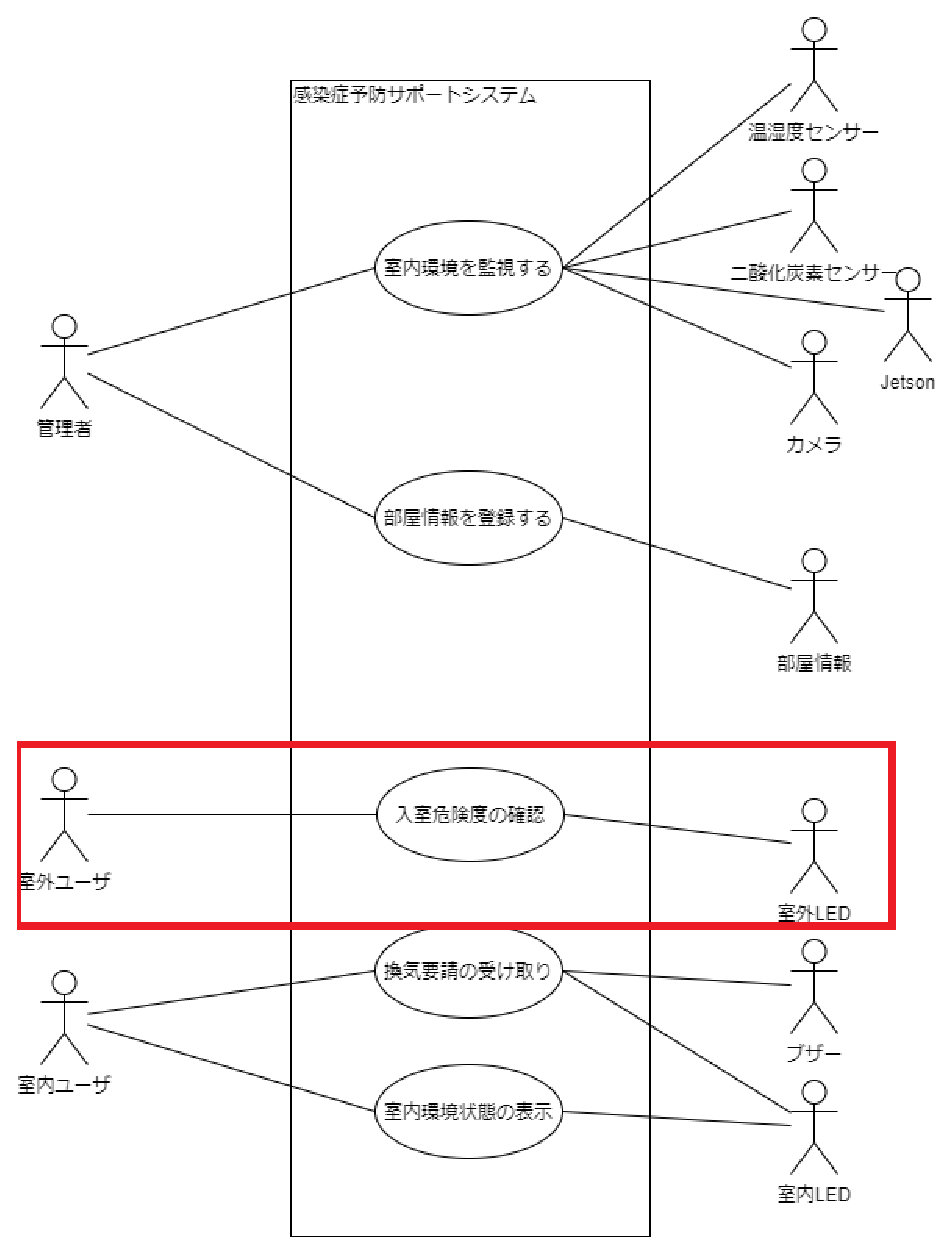
\includegraphics[width = 10cm]{./uml/usecase_e.eps}
\caption{ユースケース図}
\label{usecase1}
\end{figure}

感染症予防サポートシステムの各ユースケースについて述べる.
「室内環境を監視する」では,Webカメラにより取得した画像について人数推定を行い,室内人数に応じた監視モードを開始する.監視モードで測定した二酸化炭素濃度に応じて警戒レベルを設定し,必要に応じて換気要請を出すなどの対応をとる.
「部屋情報を登録する」では,管理者が登録した,システムを運用する部屋の広さを元に,標準警戒レベルでの滞在可能上限人数を定める.
「入室危険度の確認」では,部屋の滞在可能上限人数と現在の室内人数に応じた入室危険度を表す室外デバイスのLEDを点灯する.
「換気要請の受け取り」では,二酸化炭素濃度が各警戒レベルでの基準値を一定時間連続で超えると,LEDやブザーによって換気要請が出され,室内のユーザーは要請に従い換気を行う.
「室内環境状態の表示」では,温湿度の一定時間ごとの測定値を元に室内環境を分析し,温湿度が基準値を超えている場合は室内のLEDが点灯する.これを受けた室内のユーザーは,エアコン等により温湿度の調整を行う.
特に赤枠で囲んだ「入室危険度の確認」は筆者が実装を担当する部分となる.

上記のユースケースを受け,表\ref{sougoutestkoumoku}に示す総合テストの項目を挙げた.

\begin{table}
	\centering
	\caption{総合テスト項目}
	\label{sougoutestkoumoku}
	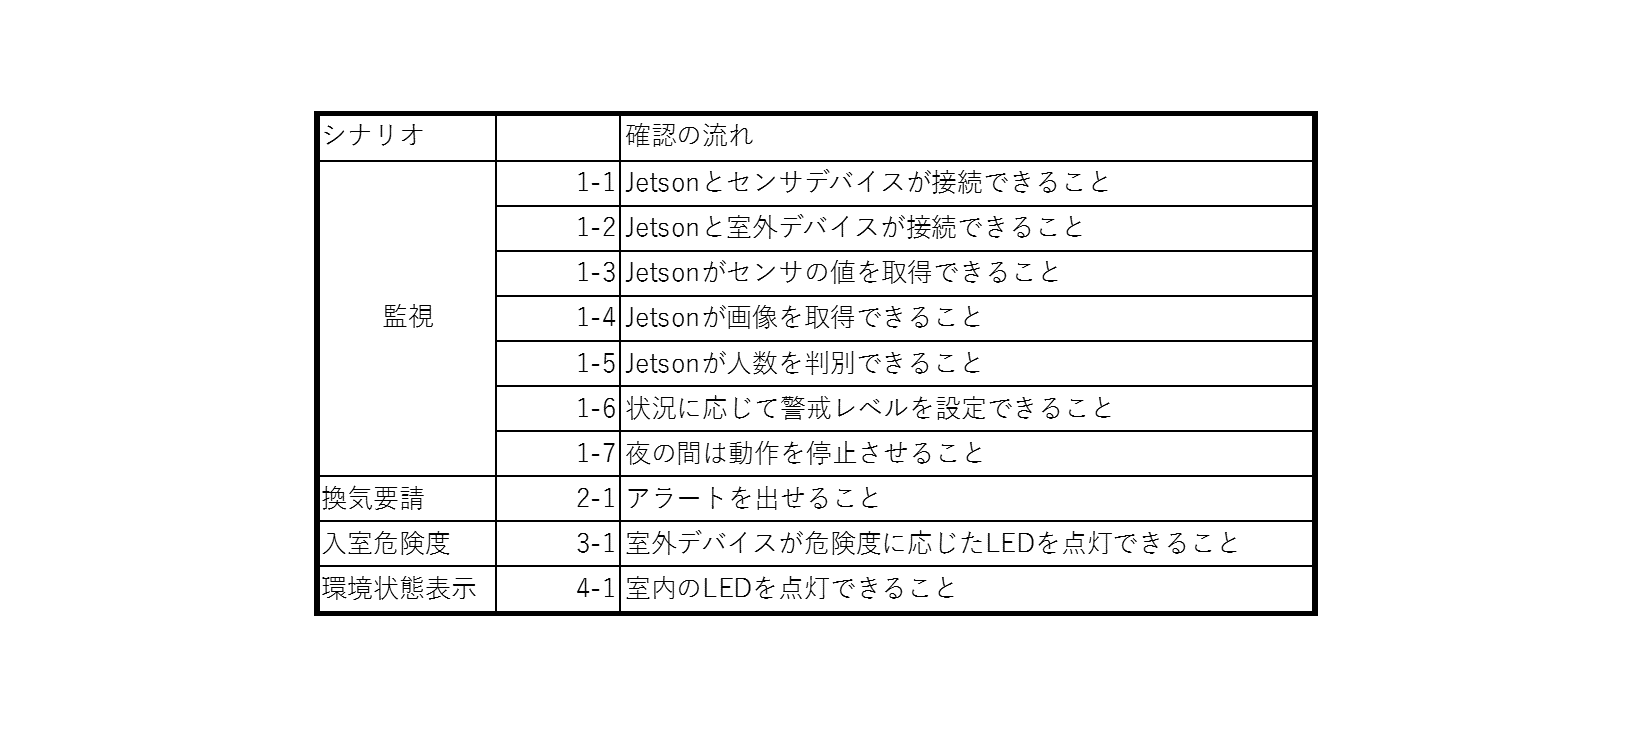
\includegraphics[width=0.9\linewidth]{test/sougoutest_koumoku}
\end{table}
\newpage
	%第3-3章
\section{基本設計}
基本設計では、ひとまとまりの処理の内容の流れを表現するために用いるアクティビティ図を作成し、「室内環境を監視する(図\ref{a_kansi})」、「換気要請の受け取り(図\ref{a_kanki})」、「入室危険度の確認(図\ref{a_nyuusitu})」、「室内環境状態の表示(図\ref{a_situnaikankyou})」の4つのユースケースについて、簡単に処理の流れを確認した。以下に作成したアクティビティ図を示す。


\begin{figure}[H]
	\centering
	\includegraphics[width=9.5cm]{a_kansi.eps}
	\caption{室内環境を監視する}
	\label{a_kansi}
\end{figure}

\begin{figure}[H]
	\centering
	\includegraphics[width=9.0cm]{a_kanki.eps}
	\caption{換気要請の受け取り}
	\label{a_kanki}
\end{figure}

\begin{figure}[H]
	\centering
	\includegraphics[width=9.5cm]{a_nyuusitu.eps}
	\caption{入室危険度の確認}
	\label{a_nyuusitu}
\end{figure}

\begin{figure}[H]
	\centering
	\includegraphics[width=10cm]{a_situnaikankyou.eps}
	\caption{室内環境状態の表示}
	\label{a_situnaikankyou}
\end{figure}

以上の4つのアクティビティ図の作成を通して、それぞれのユースケースを実現する際の処理の流れを可視化することができた。この作業を通して、ユースケース図やユースケース記述を作成した時点よりも、より論理的にシステム内部の設計を進めることができた。

上に示したアクティビティ図では、各デバイスなどのオブジェクトごとの処理のまとまりを、縦の線によってレーンとして明示的に分けて表現している。これによって、各ユースケースの全体的な処理の流れだけでなく、各ユースケースにおいて、処理やデータがオブジェクト間でどのように移されるかを確認することもできた。

具体的に見てみると、室内の複数箇所に設置するセンサデバイスは、センサから値を取得した後は、送信の機能を基本として動作すればよいことが確認できた。一方、Jetson nano側に着目すると、センサデバイスからのデータの受け取りと、室外の入室危険度表示デバイスへのデータの受け渡しというデータの流れが必要となることが確認され、Jetson nano側ではデータの送受信両方の役割を持たせなければならないことが確認できた。また、室外の入室危険度表示デバイス側は、データの取得・分析後の成果物の情報といえる、入室危険度の受け取りさえできればよいということから、受信の機能を基本として動作すればよいことを確認することができた。

アクティビティ図作成の段階では、まだ詳細な処理の流れが示されていないものの、ユースケースを実現する際の大まかな処理とデータの流れを確認することができた。また、この後の詳細設計を進める際にも、ここで作成したアクティビティ図が、基本的な考え方として活かされた。

基本設計の段階では、各デバイスがどのような振る舞いをするかを確認することができたことで、実際にシステムに用いるデバイス類の選定が可能となった。ここまでに、人数推定の機能をリアルタイム性の高い物体検出によって実現するという点から、エッジサーバ側にはJetson nanoを用いることが決まっていたが、この段階でセンサデバイス、室外の入室危険度表示デバイスに用いるデバイス類を決定した。

3.1節でも述べたが、センサデバイスは室内の複数個所に設置することを想定しており、電源の供給方法による取り付け場所の制約を受けず、なおかつ比較的低い消費電力での稼働を可能とするデバイスを選ぶ必要があった。このことから単4乾電池2本で動作し、ワイヤレスセンサーネットワークの構築に適した無線規格であるIEEE802.15.4を採用し、低消費電力での無線通信を可能にする無線マイコンモジュールとしてTWELITEを選定し、室外に設置する部屋への入室の危険度を表示するデバイスに関しても、同じくTWELITEを選定した。また、Jetson nanoにもこのTWE-LITEをUARTによって接続し、センサデバイスとしてのTWE-LITEや、室外の入室危険度表示デバイスとしてのTWE-LITEそれぞれとの通信を可能とし、エッジサーバとして必要となる、データ送受信の機能を持たせている。

ここまでの設計内容をもとにクラス図を作成したところ、図\ref{class}のように本システムの静的な構造が確認できた。ただし、3.4節でも述べるがJetson nano側では、センサデバイスから受け取ったデータを管理するために、データベースを用いることとしている。

\begin{figure}[H]
	\centering
	\includegraphics[width=12cm]{class.eps}
	\caption{クラス図}
	\label{class}
\end{figure}


また、以上の基本設計の内容をもとに、結合テスト項目として表\ref{ketugoutest_koumoku}の項目を挙げた。


\begin{table}[H]
	\centering
	\caption{結合テスト項目}
	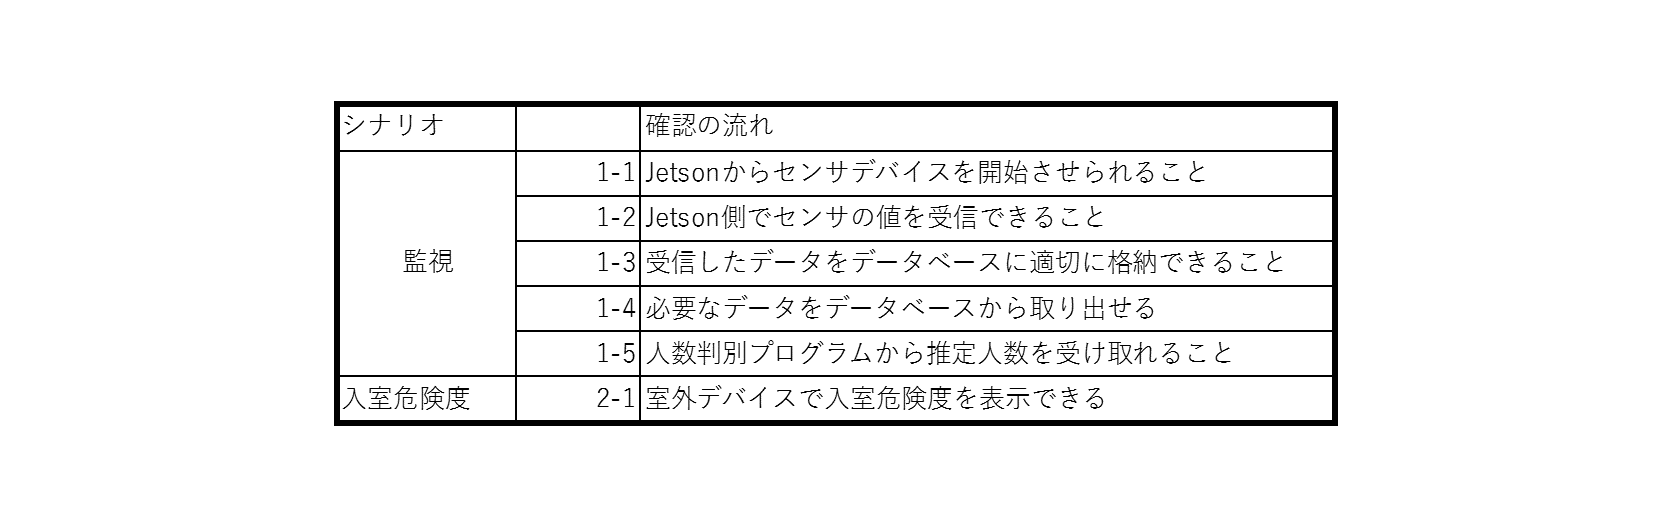
\includegraphics[width=15cm]{ketugoutest_koumoku.eps}
	\label{ketugoutest_koumoku}
\end{table}




	
\section{使用部品の選定(TWELITE)}

基本設計の段階において,筆者が担当した室外デバイスで使用する部品の選定を行った.
室外デバイスのマイコンについては,モノワイヤレス株式会社の無線マイコンであるTWELITEを使用した\cite{twelite}.
室外デバイスはJetsonと通信する必要があり,また,コードの配線を考えずに済むように無線通信ができるマイコンを採用することとした.
さらに設置場所の制約を少なくするため,室外デバイスはできるだけサイズを小さくしたい.このため,マイコンボードに無線機能があらかじめ実装されているもの,乾電池で動作できるものを採用することとした.ただし,乾電池の一般的な起電力である1.5Vで動作するマイコンボードはほとんどないため,ここでは乾電池を2本使用して3Vで動作するものとする.
以上の理由より,起電力3Vで動作し,無線機能があらかじめ実装されているTWELITEを選定した.
今回使用したのはTWELITE DIP BLUEである(図\ref{tweblue}).以下の表\ref{siyou}に仕様を示す.

\begin{figure}
	\centering
	\includegraphics[width=0.3\linewidth]{tweblue}
	\caption{TWELITE DIP BLUE}
	\label{tweblue}
\end{figure}

\begin{table}
	\centering
	\caption{TWELITE DIP BLUEの仕様}
	\begin{tabular}{|c|c|}
		\hline
		送信出力 & +2.50dBm \\
		\hline
		受信感度 & -95dBm \\
		\hline
		送信電流 & 15.3mA (+2.50dBm出力時) \\
		\hline
		受信電流 & 17.0mA \\
		\hline
		外形寸法 & 35.7mm x 17.7mm x 3.5mm \\
		
		& (アンテナ,コネクタ,端子除く) \\
		\hline
		& 3.6g (マッチ棒アンテナ版) \\
		
		重量 & 3.7g (同軸コネクタ版) \\
		
		& (アンテナ,コネクタ,端子除く) \\
		\hline
		動作電圧 & 2.3~3.6V \\
		\hline
		動作温度 & -40~85℃ \\
		\hline
		電波認証 & ARIB STD-T66 (技適) \\
		\hline
	\end{tabular}
	\label{siyou}
\end{table}
\newpage
	%第3章

\section{詳細設計}

オブジェクト間のメッセージのやりとりを時系列に沿って表現するために,以下に示すシーケンス図を作成した.
換気要請についてのシーケンス図を図\ref{sequencekanki}に,室内の監視についてのシーケンス図を図\ref{sequencekanshi}に,室内環境についてのシーケンス図を図\ref{sequenceshitsunai}に,入室危険度についてのシーケンス図を図\ref{sequencenyushitsu}に示す.

\begin{figure}
	\centering
	\includegraphics[width=15cm]{./uml/sequence_kanki_2}
	\caption{換気要請についてのシーケンス図}
	\label{sequencekanki}
\end{figure}

「換気要請」について,まずセンサデバイスが3分経過ごとに二酸化炭素センサへ値の取得指示を出す.
取得した二酸化炭素濃度をJetsonへ送信し,Jetsonはセンサデータベースへデータを記録した後,15分間分のデータをデータベースから取得する.
次にカメラから画像を取得し人数推定を行う.推定した人数と取得した二酸化炭素濃度値を,警戒レベルが保有する上限人数と二酸化炭素濃度の基準値と比較し換気要請の判断を行う.その後換気要請に応じてLEDとブザーに指示を出す.

\begin{figure}
	\centering
	\includegraphics[width=15cm]{uml/sequence_kanshi_3}
	\caption{室内の監視についてのシーケンス図}
	\label{sequencekanshi}
\end{figure}

「室内の監視」について,システムを起動するとJetsonはセンサデバイスへ開始の指示を行う.
指示を受けたセンサデバイスは二酸化炭素センサへ値の取得指示を出す.
その後はセンサデバイスが3分経過ごとに二酸化炭素センサへ値の取得指示を出し,人数推定を行うまで「換気要請」の場合と同様であり,
推定した人数と取得した二酸化炭素濃度値を,警戒レベルが保有する上限人数と二酸化炭素濃度の基準値と比較し,警戒レベルを設定する.

\begin{figure}
	\centering
	\includegraphics[width=15cm]{uml/sequence_shitsunai_2}
	\caption{室内環境についてのシーケンス図}
	\label{sequenceshitsunai}
\end{figure}

「室内環境」について,まずセンサデバイスが3分経過ごとに温湿度センサへ値の取得指示を出す.
取得した温湿度をJetsonへ送信し,Jetsonはセンサデータベースへデータを記録した後,これまでの温湿度データを取得する.
温湿度の平均値を算出し,適正範囲内か否かによって温湿度アラートLEDを制御する.

\begin{figure}[htbp]
\centering
\includegraphics[width=15cm]{./uml/sequence_nyushitsu_e.eps}
\caption{入室危険度についてのシーケンス図}
\label{sequencenyushitsu}
\end{figure}

「入室危険度」について,人数推定を行うまでは「換気要請」等と同様の流れである.
その後,現在の室内滞在人数と,警戒レベルが保有する滞在上限人数,滞在推奨人数を比較し入室危険度を決定する.
Jetsonから室外デバイスに入室危険度を送信し,室外デバイスは入室危険度に応じてLEDの制御を行う.
赤枠で囲んだ屋外デバイスとLEDは筆者が実装を担当する.

次に,筆者が実装を担当した室外デバイスのステートチャート図を図\ref{statechartokugai}に示す.

\begin{figure}
	\centering
	\includegraphics[width=0.3\linewidth]{uml/statechart_okugai_1}
	\caption{室外デバイスのステートチャート図}
	\label{statechartokugai}
\end{figure}

室外デバイスはシステムが稼働している間,常に入室危険度の受信待機状態であり,Jetsonから入室危険度が送られてきた場合に入室危険度に応じた色のLEDが点灯する.

以上の詳細設計より表\ref{tantaitestsitsugaikoumoku}に示す室外デバイスにおける単体テスト項目を挙げた.

\begin{table}
	\centering
	\caption{室外デバイスにおける単体テスト項目}
	\label{tantaitestsitsugaikoumoku}
	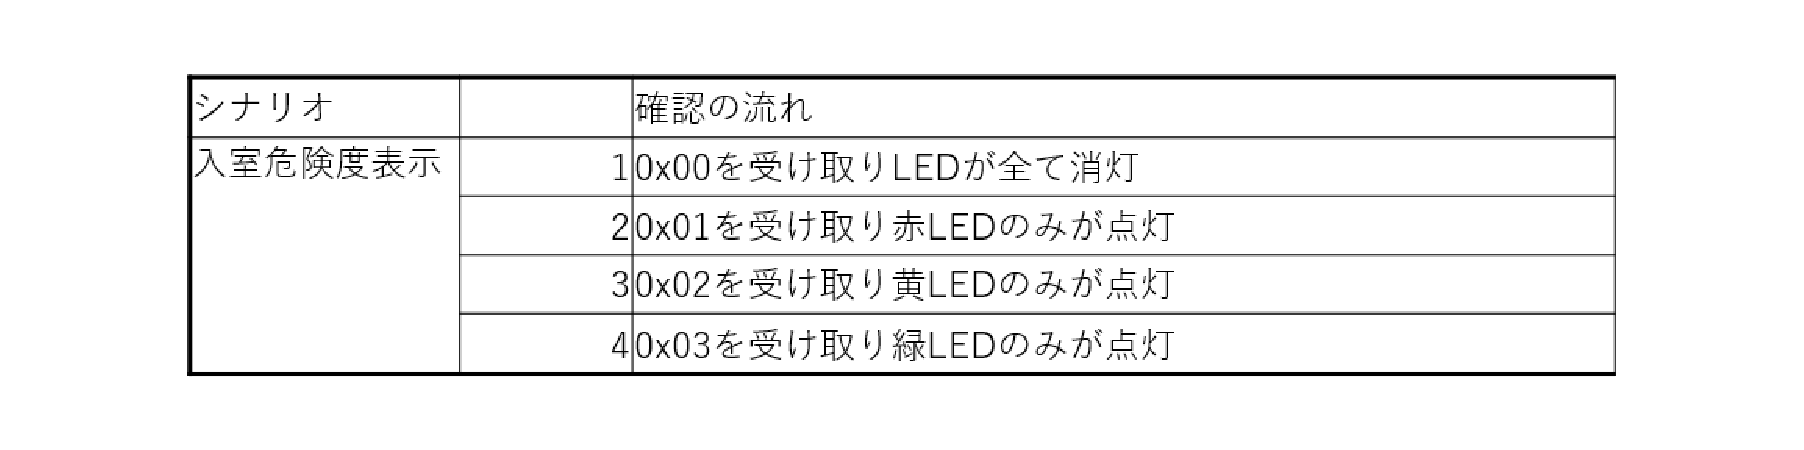
\includegraphics[width=0.9\linewidth]{test/tantaitest_sitsugai_koumoku2}
\end{table}
	
	%第4章
	\chapter{実装・検証}
	%第4章:システム仕様

本章では,SAS-L2を用いたセキュアな組込みシステムについての仕様を述べる.

\section{SAS-L2を用いたセキュアな組込みシステムの概要}
はじめに,SAS-L2を利用したセキュアな組込みシステムの概要図を図\ref{fig:gaiyo}示す.

\begin{figure}[H]
\begin{center}
	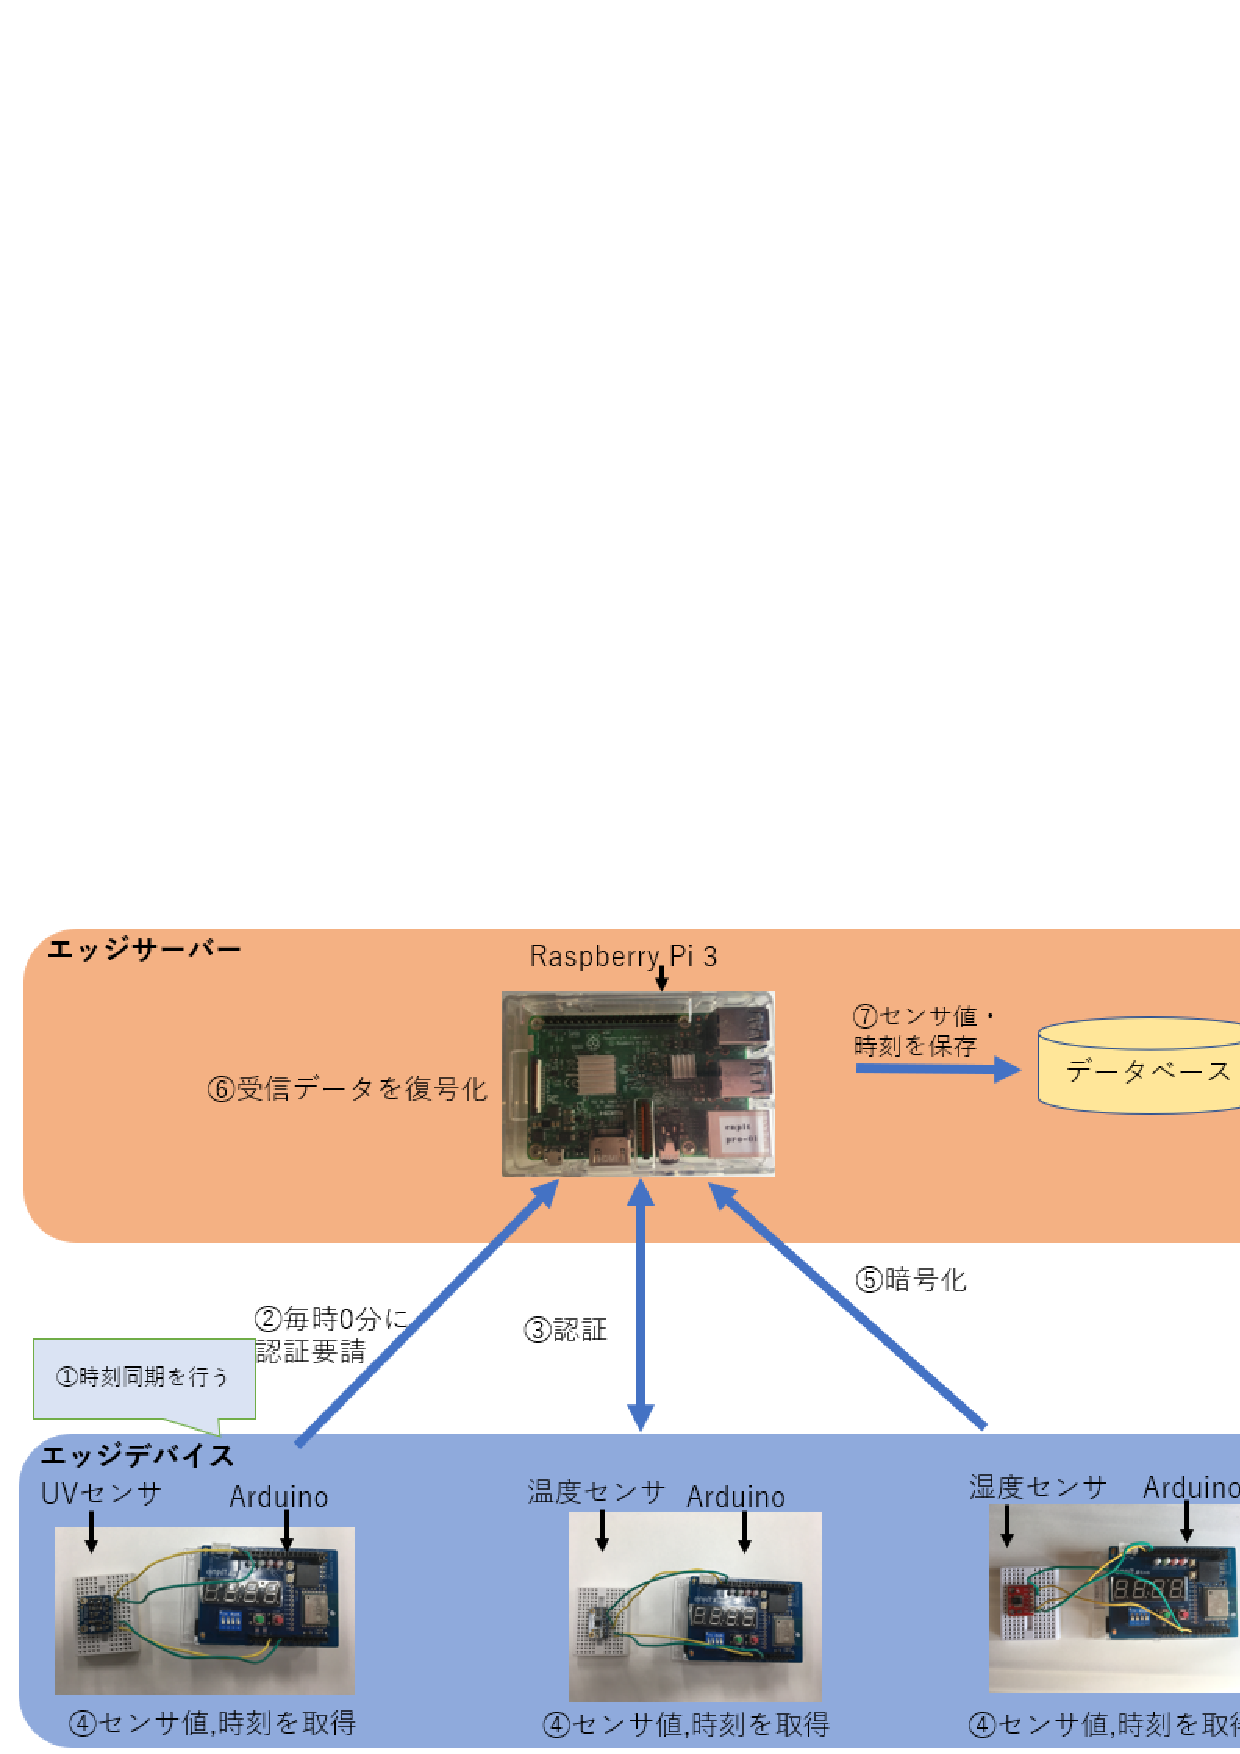
\includegraphics[height=80mm]{gaiyo.png}
	\caption{SAS-L2を利用したセキュアな組込みシステムの概要図}
\label{fig:gaiyo}
\end{center}
\end{figure}

Raspberry Piをエッジサーバーとし,3台のArduinoをエッジデバイスとして利用する.
図\ref{fig:gaiyo}のように,エッジデバイスにはそれぞれ,UVセンサ,温度センサ,湿度センサを接続している.
データベースには,エッジデバイスから収集したデータを保存する.
以降,エッジサーバーをサーバー,エッジデバイスをユーザーと定義する.
図\ref{fig:gaiyo}に沿って,SAS-L2を利用したセキュアな組込みシステムの時刻同期,センシングデータ取得,認証,および暗号化通信の処理の流れを説明する.

\begin{enumerate}
	\item ユーザーを起動し,時刻同期を行う.
	\item ユーザーはサーバーに対して,指定した時刻に認証要請を行う.
	\item サーバーは認証要請を受信し,認証要請を送信したユーザーとのSAS-L2認証を行う.
	\item ユーザーは認証完了後,接続されたセンサからセンシングデータ(センサ値)と,
    センシングデータを取得した日時を取得する.
	\item ユーザーは処理4で取得したデータを暗号化しサーバーへ送信する.
	\item サーバーはユーザーから受信したデータを復号し,センシングデータと日時を取得する.
    \item サーバーは取得した,センシングデータと日時をデータベースに保存する.
    \item 処理4から処理7を10回繰り返す.
    \item 処理2から処理8を繰り返す.
\end{enumerate} 

以上のように,指定した時刻になると認証1回,暗号化通信10回を行うシステムとなる.

\section{要件定義}
SAS-L2を利用したセキュアな組込みシステムの要件定義を述べる.
要件定義には,機能要件と非機能要件がある.
機能要件は,システムで実現すべき機能であり,クライアントから求められる機能のことである.
非機能要件は,機能要件以外の要件であり,主に性能やセキュリティ,環境,制約を指す.
\subsubsection{機能要件}
\begin{enumerate}
	\item 指定した時刻にユーザ―からサーバーにコネクションして認証要請を送信する.
	\item サーバーとユーザー間でSAS-L2による認証を行う.
    \item 認証が成功した場合,サーバーとユーザー間でSAS-L2に基づいた暗号化通信を行う.
    \item 認証が失敗した場合,コネクションを切断してシステム概要で述べた処理1からやり直す.
	\item サーバーは受信データを復号してセンシングデータと日時をデータベースへ保存する.
    \item 暗号化通信終了後,サーバーはコネクションを切断し,ユーザーからの認証要請待ち状態となる.
\end{enumerate} 

\subsubsection{非機能要件}
\begin{enumerate}
    \item 複数のユーザーは同時刻に認証要請を送信するので,一台の認証が終了するまで,その他のユーザーは待機状態になる.
    \item サーバーは認証結果をユーザーに送信する.
    \item サーバーとユーザーは認証結果を表示する.
    \item ユーザーは,シリアルモニタに取得したセンシングデータとセンシングデータの取得日時を表示する.
    \item ユーザーは起動後,1度時刻同期を行う.
    \item サーバーは暗号化通信の際,5秒以上データを受信できなければ,コネクションを切断し,認証要請受信の待機状態となる.
	\item 指定した時刻毎に3つのユーザーとの通信を10秒以内に終わらせる.
    \item サーバーはセンシングデータと取得日時を保存する際に,ユーザーごとのテーブルに分けて保存する.
    \item 1度の認証につき,10回の暗号化通信を行う.
	\item ユーザーで,何らかのエラーが発生した場合,赤LEDを点滅させる.
\end{enumerate} 

	%第4-1章:実装

\section{実装}

第3章で述べたシステム全体の機能はグループで実装を行い,筆者は室外表示用のデバイスの実装を担当した.
室外デバイスの動作としては,Jetsonから入室危険度を受信し,入室危険度に応じたLEDの制御を行うというものである.
また,第3章でも述べたように,無線マイコンとしてTWELITEを用いて実装を行った.
マイコンボード上で動作するソフトウェアについては,TWELITE MWX ライブラリを利用し,C++言語を用いて開発を行った.
図\ref{zikki}が実際に作成した室外デバイスである.

\begin{figure}
	\centering
	\includegraphics[width=0.5\linewidth]{zikki}
	\caption{作成した室外デバイス}
	\label{zikki}
\end{figure}

筆者が担当する室外表示デバイスに対して単体テストを行った.その後,グループメンバーが開発した機能部と合わせて結合テストと総合テストを行った.以下,検証項目について述べる.
	%第4章:検証

\section{検証}

\subsection{単体テスト}

詳細設計の際に挙げた単体テストの項目に従って単体テストを行った.単体テストの結果を表\ref{tantaitestsitsugaikekka}に示す.

\begin{table}
	\centering
	\caption{室外デバイスの単体テストの結果}
	\label{tantaitestsitsugaikekka}
	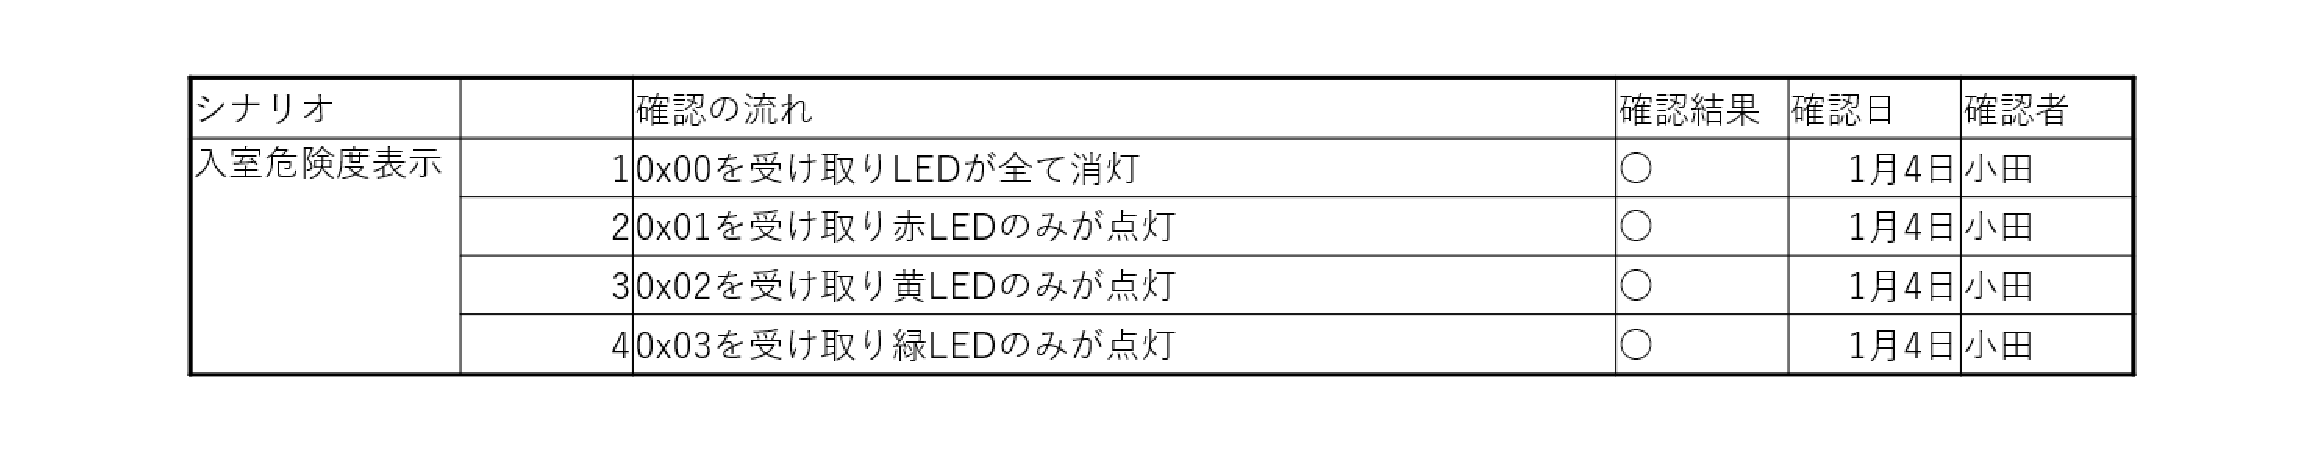
\includegraphics[width=0.9\linewidth]{test/tantaitest_sitsugai_kekka2}
\end{table}

単体テストの実施においては,TWELITEのUART接続を用いてデバイスをPCに接続して行った.
単体テスト項目1~4までPC上から室外デバイスにコマンドを送り,すべて消灯した状態と各入室危険度を表すLEDの制御が正しくできることを確認した.

\subsection{結合テスト}

基本設計の際に挙げた結合テストの項目に従って結合テストを行った.結合テストの結果を表\ref{ketugoutest}に示す.

\begin{table}
	\centering
	\caption{結合テストの結果}
	\label{ketugoutest}
	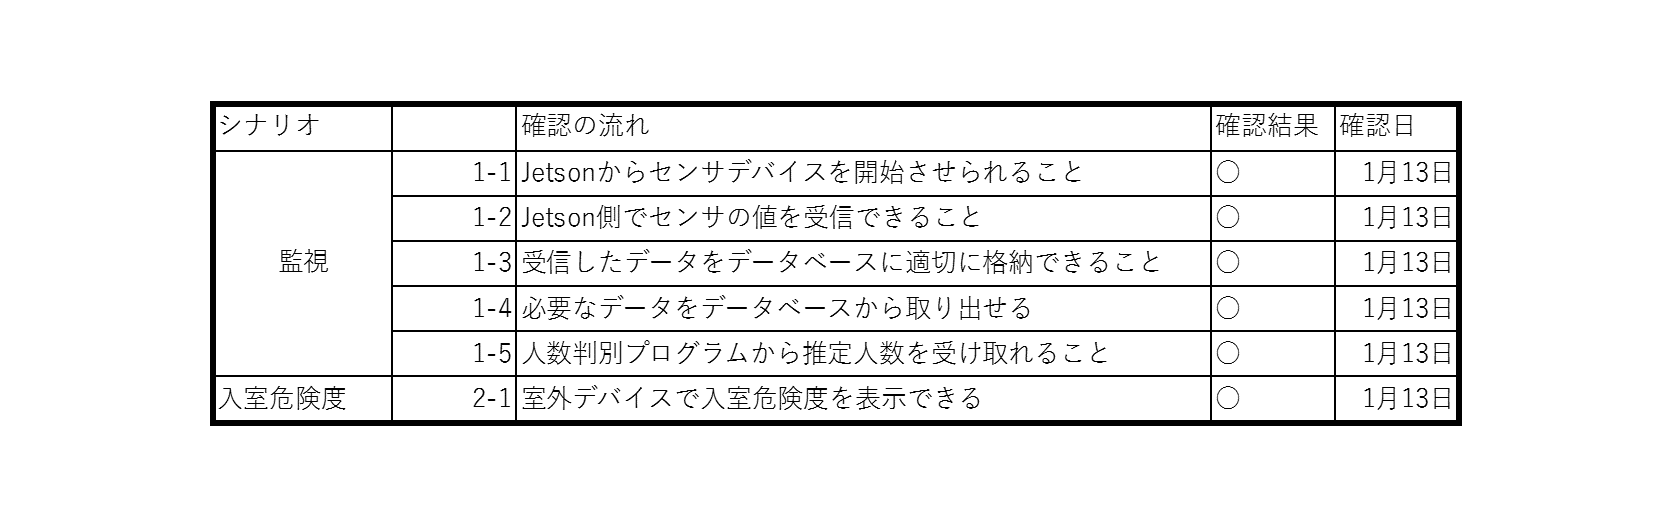
\includegraphics[width=0.9\linewidth]{test/ketugoutest}
\end{table}

結合テストは,環境値評価と人数推定を同一プログラムで行える状態で,データベース操作のプログラムも同一のJetsonで行えるようにして状態で実施した.

項目1-1については,センサデバイスの電源が入っている状態でJetsonの処理プログラムを開始したところ,LEDの状態変化によりセンサデバイスが正しく動作することを確認した.
項目1-2については,Jetsonの処理プログラムを実行することでセンサデバイスから電波を受信していることを確認した.
項目1-3については,処理プログラムの動作中にデータベースに格納された値を定期的に確認し,受信したデータを適切に格納できていることを確認した.
項目1-4については,データベースにデータが格納されている状態から,その値を用いた評価ができていることを確認した.
項目1-5については,プログラムの中で人数推定の結果を正しく受け取れていることを確認した.
項目2-1については,Jetson上で評価した入室危険度に応じて室外デバイスのLEDが正しく点灯していることを確認した.

\subsection{総合テスト}

要求定義の際に挙げた総合テストの項目に従って総合テストを行った.総合テストの結果を表\ref{sougoutest}に示す.

\begin{table}
	\centering
	\caption{総合テストの結果}
	\label{sougoutest}
	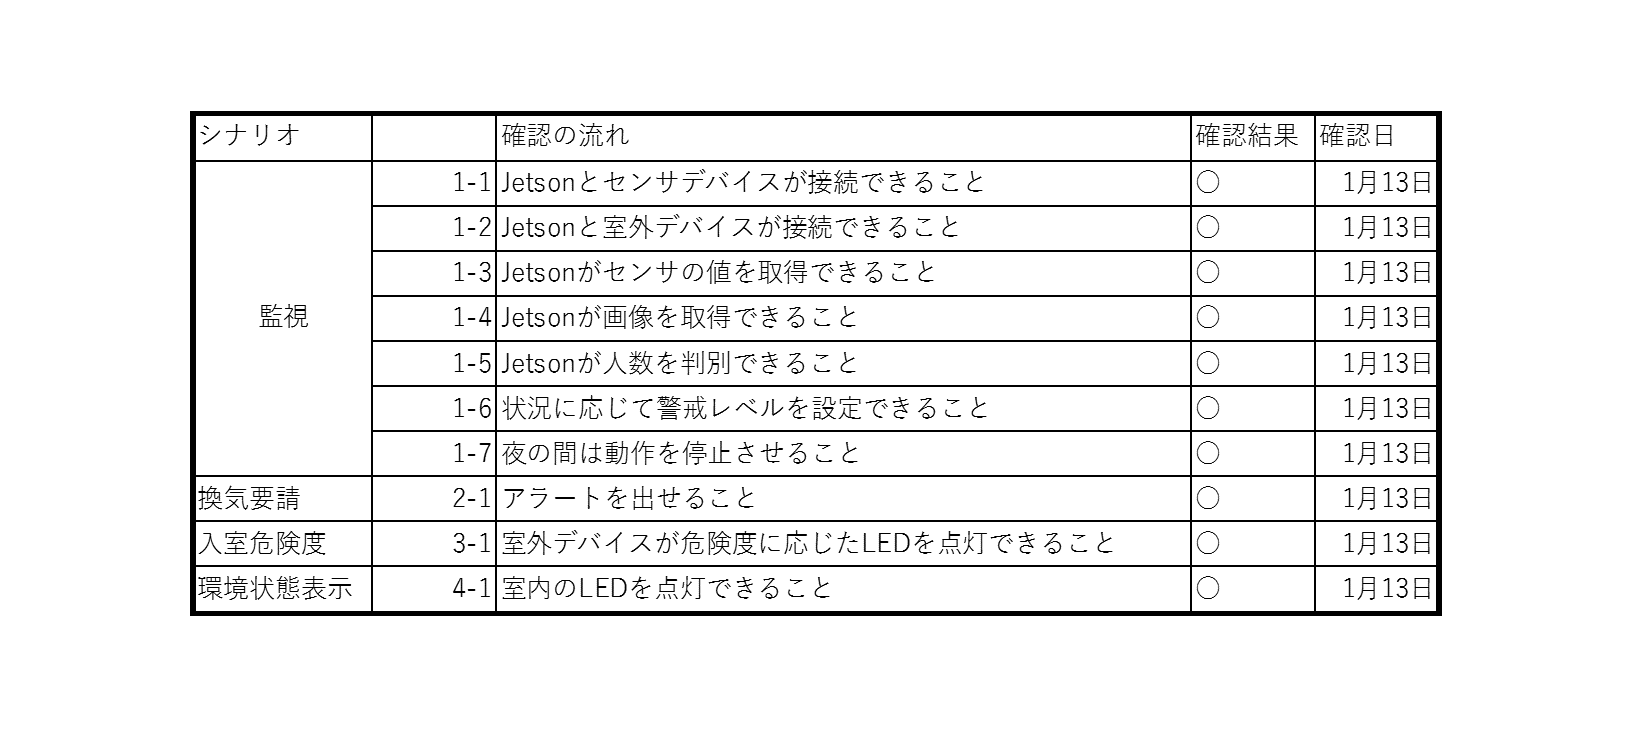
\includegraphics[width=0.9\linewidth]{test/sougoutest}
\end{table}

総合テストは実際にシステムの利用を想定した環境で行った.
項目1-1については,システム実行時にセンサデバイスがJetsonからの開始信号を受け取ることでLEDの状態が変化し,Jetsonとセンサデバイスが接続できていることを確認した.
項目1-2については,システム実行時に室外デバイスのLEDがすべて消灯されるようにすることで,Jetsonと室外デバイスが接続できていることを確認した.
項目1-3については,Jetsonがセンサデバイスから値を受信し,その後の処理に利用できていることを確認した.
項目1-4については,JetsonがWebカメラから画像を取得し,その画像をJetsonと接続したPC上に表示することで正しく画像が取得できていることを確認した.
項目1-5については,人数の異なる集合写真を用いて人数推定を行い,おおむね正しく人数判別できていることを確認した.
項目1-6については,人数の多い集合写真を用いて,室内滞在人数が多く,二酸化炭素濃度値が基準値より高い場合に警戒レベルが上がっていることを確認した.
同様にして,項目2-1と項目4-1について,換気要請のブザーや室内LEDが正しく動作することを確認した.
項目1-7については,設定した時間中,センサ値の取得およびシステムの処理が中断されることを確認した.
項目3-1については,Jetsonが評価した入室危険度に応じて室外デバイスのLEDが正しく点灯することを確認した.
	
	%第5章
	\chapter{評価・考察}
	%第5章
本章では、本システムに対する評価・考察を行い、今後の課題や将来性についても述べる。

まず3.1節に挙げた、本システムが果たすべき2つの大きな役割に対して評価する。3.1節において、本システムが果たすべき役割について、「感染症予防対策のルールを守ってもらうよう働きかける役割」、「感染症予防対策の基準を定める役割」の2つを挙げた。感染症予防対策のルールを守ってもらうよう働きかける役割については、室内環境に応じた換気要請の発出や、感染リスクのレベルの通知によって、換気や人数調整といった具体的なアクションを促すことが実現できていると考えられる。感染症予防対策の基準を定める役割については、利用者が感染症予防のためにとるべき、換気と部屋に滞在する人数の調整というアクションについて、感染症予防の観点から、部屋を安全な状態に保つため、具体的にその基準を定めることで、利用者自身が感染症予防のためにとるべきアクションを明確にすることが実現できていると考えられる。

また本システムでは、センサデバイスで取得したデータを随時データベースに記録しているほか、室内の滞在人数や警戒レベル、感染リスクといったデータも、センサデバイスからのデータ更新に伴って導き出されていることから、必要に応じてデータを保管しておくことで、システム外部で様々なデータの相関を調べることもできる。そのため、感染症予防対策の基準を定める役割に関しては、応用の余地があると考えられ、例えば以下のような応用の仕方が考えられる。

本システムでは、分析に活かせる多くのデータを導き出せるが、中でも設計の段階から分析に役立てられるデータとして着目していたのは、警戒レベルと感染リスクのデータである。既に述べたように、室内にある程度の人数が滞在していないと警戒レベルの導出は行われない。そのため警戒レベルの推移のデータは、その部屋が警戒レベルを導出できる条件下で利用されているとき、どの程度二酸化炭素濃度が高まりやすいかを確認でき、運用ルール改定の基準にできる。また、警戒レベルと感染リスクのデータをシステム内部で分析し、本システムでは固定的である、二酸化炭素濃度と警戒レベル、警戒レベルと滞在可能人数の関係を、部屋の警戒レベルと感染リスクの変動の仕方に応じて流動的に変化させると、よりその部屋にあった感染症予防対策を講じることが可能になると考えられる。

感染リスクのデータは、換気状況など、部屋の運用の仕方が適切であるかどうかを示しているため、部屋が感染症予防対策上、危険な状態で使用されていないかを確認できる。そのため学校やオフィス、公共施設などでの利用のケースを想定すると、時間帯ごとの感染症予防対策への取り組みの徹底度合いが、エビデンスとして残されることから、管理者側からの適切な指導が行えるほか、各部屋の責任者となる者が、感染症予防対策に、より注意して取り組むことができると考える。

本システムの設計時の着想では、利用環境ごとに異なる、床面積の広さ・空間の広さ、換気のしやすさや窓の位置と数、換気設備の有無、部屋利用者の活動の仕方などに柔軟に対応し、利用環境に合わせた感染症予防対策の基準を定め、利用者に感染症予防対策のルールを守ってもらうよう働きかけられることが本システムの特徴であった。実際に、本システムは4.2節の総合テストでの検証のように、様々なシナリオにあった感染症予防の働きかけが可能となることが考えられる。しかしながら、本システムでの感染症予防対策の基準の決め方では、換気のしやすさや、部屋の床面積の広さのわりに、ものが多く置かれているなどの理由から実際の空間が狭いというような部屋の特性が、そのまま二酸化炭素濃度の上昇の仕方に反映されることを前提としている部分があり、柔軟性に欠けていると考える。理想的な環境における本システムの実用性は確認されたものの、部屋ごとの特性を加味した感染症予防対策の基準を、実際の利用環境において適切に定めるためには、本システムでの室内環境の分析の仕方よりも複雑に、室内環境を分析する必要があるとも考えられ、部屋の特性自体をシステムの分析機能によって導き出すことができると、現在のシステムと比較し、よりその部屋の特性に適合した感染症予防対策の基準の設定を行うことができるため、更なる研究と改良の余地が大いに残されていると考える。



	%第5-1章:評価

\section{評価}

第3章では,感染症予防サポートシステムは,感染症予防の観点から感染リスクのレベルを通知するとともに,感染リスクを軽減する環境づくりをサポートするという目的を基にして,下記の2点の要求事項を満たす必要があるとした.

\begin{itemize}
	\item 室内環境が測定できること.
	\item 設定した感染リスクの基準に従って通知ができること.
\end{itemize}

「室内環境が測定できること」という要求事項に関して,作成したシステムは二酸化炭素濃度,温湿度,室内滞在人数の測定ができるため,要求を満たすことができたといえる.
「設定した感染リスクの基準に従って通知ができること」という要求事項に関しては,警戒レベル,換気要請の基準,入室危険度を設定し,警戒レベルおよび入室危険度はLED,換気要請はブザーによって,ユーザーに感染リスクの情報を,視覚や聴覚で分かりやすく能動的に通知することができた.室外のユーザーには室外デバイスによるLEDでの入室危険度の通知,室内のユーザーにはブザーとLEDによる換気要請や警戒レベルの通知というように,対象とするユーザーによって提供する情報,提供の方法を変えることで,室内外から共に感染リスクを軽減する環境づくりをサポートするシステムとなった。
	%第5章:考察

\section{考察}

今回作成した感染リスク通知デバイスは3色のLEDで入室危険度を分かりやすく表示するというものである.
理想的には,センサーとカメラで収集した施設内の環境情報(在室人数,入室できる人数,二酸化炭素濃度水準,換気状態,感染リスク等の情報)を利用者対象別に提供することが望ましいが,ハードや時間の制約のために,室内外への感染リスクに関する基本的な情報提供機能のみの実装となり,すべての環境情報をユーザーに知らせるまで至らなかった.
しかしながら,在室人数,入室可能人数,二酸化炭素濃度等の数値に関して,本システムはデータを収集できている.
今後,ディスプレイ等を使用すれば,Jetsonから各種データを受け取ることで室内外により詳細な環境情報を表示することができると考える.

	
	%第6章
	\chapter{あとがき}
	%あとがき
本研究ではセンシング技術、物体検出技術、および複数デバイス間の無線通信という3つの技術とデータ分析の組み合わせによって、感染症予防という、研究・実用化が活発に進められる分野において新たな価値を生み出すことができた。感染症予防に関しては、既に様々な分野で研究・開発がなされているものと思われるが、今回私たちが開発したシステムも、感染症予防の取組を援用するシステムとして貢献できると考える。

また今回の研究では、感染症予防のために活用できるシステムの社会的な必要性が高まり、多くの企業や研究機関により研究・開発が進められている状況下で、感染症予防のために用いるシステムとして、3 密回避に役立てられるという、新型コロナウイルスの世界的な流行以前にはなかった新しい価値を持たせることも、1つの目標として定められた。本研究において、私たちの考える感染症予防のサポートシステムの基本形を提案することができた。今後さらなる研究が進められれば、より高いリアルタイム性と精度を併せ持つモニタリングと、感染症予防対策基準の設定機能における更なる柔軟性を実現でき、より利用しやすいものへと改良が進められることから、拡張性のある研究であると考える。

	%--ここまで本文--
	
	
	%謝辞
	\newpage
	\addcontentsline{toc}{chapter}{\protect\numberline{謝辞}{}}
	\chapter*{謝辞}
	%--ここから謝辞--
	本研究を進めるにあたり,懇篤な御指導,御鞭撻を賜わりました本学高橋寛教授に深く御礼申し上げます.
	
	本論文の作成に関し,詳細なるご検討,貴重な御教示を頂きました本学甲斐博准教授ならびに王森レイ講師に深く御礼申し上げます.
	
	本研究に際しご審査いただきました稲元 勉講師,井門 俊講師に深く御礼申し上げます.
	
	最後に,多大な御協力と貴重な御助言を頂いた本学工学部情報工学科情報システム工学講座高橋研究室の諸氏に厚く御礼申し上げます.
	
	%--ここまで謝辞--
	
	%参考文献
	\begin{thebibliography}{99}
		%ここから参考文献
		
		\bibitem{qa}
		厚生労働省,新型コロナウィルスに関するQ\&A(一般の方向け)$|$厚生労働省,
		https://www.mhlw.go.jp/stf/seisakunitsuite/bunya/kenkou\_iryou/\\dengue\_fever\_qa\_00001.html,2021-1-4
		
		\bibitem{kanki}
		厚生労働省,「換気の悪い密閉空間」を改善するための換気の方法,
		https://www.mhlw.go.jp/content/10900000/000618969.pdf,2020-4-3
		
		\bibitem{isence}
		中畑和之,森伸一郎,板垣吉晃,河合慶有, "コロナウイルス対策のための教室換気実験とアラートシステムの構築," 愛媛大学工学部社会基盤iセンシングセンター報告資料,  2020年11月.
		
		\bibitem{vji}
		V字モデル(V-model)とは -IT用語辞典 e-Words,
		https://e-words.jp/w/V%E5%AD%97%E3%83%A2%E3%83%87%E3%83%AB.html
		
		\bibitem{uml}
		株式会社 オージス総研, かんたんUML[増補改訂版], 翔泳社, 2003
		
		\bibitem{twelite}
		モノをつなぐ無線マイコンモジュール TWELITE-トワイライト - MONO-WIRELESS.COM,
		https://mono-wireless.com/jp/products/TWE-LITE/index.html
		%ここまで参考文献
		
	\end{thebibliography}
\end{document}
